\PassOptionsToPackage{unicode=true}{hyperref} % options for packages loaded elsewhere
\PassOptionsToPackage{hyphens}{url}
%
\documentclass[english,man]{apa6}
\usepackage{lmodern}
\usepackage{amssymb,amsmath}
\usepackage{ifxetex,ifluatex}
\usepackage{fixltx2e} % provides \textsubscript
\ifnum 0\ifxetex 1\fi\ifluatex 1\fi=0 % if pdftex
  \usepackage[T1]{fontenc}
  \usepackage[utf8]{inputenc}
  \usepackage{textcomp} % provides euro and other symbols
\else % if luatex or xelatex
  \usepackage{unicode-math}
  \defaultfontfeatures{Ligatures=TeX,Scale=MatchLowercase}
\fi
% use upquote if available, for straight quotes in verbatim environments
\IfFileExists{upquote.sty}{\usepackage{upquote}}{}
% use microtype if available
\IfFileExists{microtype.sty}{%
\usepackage[]{microtype}
\UseMicrotypeSet[protrusion]{basicmath} % disable protrusion for tt fonts
}{}
\IfFileExists{parskip.sty}{%
\usepackage{parskip}
}{% else
\setlength{\parindent}{0pt}
\setlength{\parskip}{6pt plus 2pt minus 1pt}
}
\usepackage{hyperref}
\hypersetup{
            pdftitle={Experience with research paradigms relates to infants' direction of preference.},
            pdfkeywords={preference, looking, paradigm, novelty, infants},
            pdfborder={0 0 0},
            breaklinks=true}
\urlstyle{same}  % don't use monospace font for urls
\usepackage{longtable,booktabs}
% Fix footnotes in tables (requires footnote package)
\IfFileExists{footnote.sty}{\usepackage{footnote}\makesavenoteenv{longtable}}{}
\usepackage{graphicx,grffile}
\makeatletter
\def\maxwidth{\ifdim\Gin@nat@width>\linewidth\linewidth\else\Gin@nat@width\fi}
\def\maxheight{\ifdim\Gin@nat@height>\textheight\textheight\else\Gin@nat@height\fi}
\makeatother
% Scale images if necessary, so that they will not overflow the page
% margins by default, and it is still possible to overwrite the defaults
% using explicit options in \includegraphics[width, height, ...]{}
\setkeys{Gin}{width=\maxwidth,height=\maxheight,keepaspectratio}
\setlength{\emergencystretch}{3em}  % prevent overfull lines
\providecommand{\tightlist}{%
  \setlength{\itemsep}{0pt}\setlength{\parskip}{0pt}}
\setcounter{secnumdepth}{0}

% set default figure placement to htbp
\makeatletter
\def\fps@figure{htbp}
\makeatother

% Manuscript styling
\usepackage{upgreek}
\captionsetup{font=singlespacing,justification=justified}

% Table formatting
\usepackage{longtable}
\usepackage{lscape}
% \usepackage[counterclockwise]{rotating}   % Landscape page setup for large tables
\usepackage{multirow}		% Table styling
\usepackage{tabularx}		% Control Column width
\usepackage[flushleft]{threeparttable}	% Allows for three part tables with a specified notes section
\usepackage{threeparttablex}            % Lets threeparttable work with longtable

% Create new environments so endfloat can handle them
% \newenvironment{ltable}
%   {\begin{landscape}\begin{center}\begin{threeparttable}}
%   {\end{threeparttable}\end{center}\end{landscape}}
\newenvironment{lltable}{\begin{landscape}\begin{center}\begin{ThreePartTable}}{\end{ThreePartTable}\end{center}\end{landscape}}

% Enables adjusting longtable caption width to table width
% Solution found at http://golatex.de/longtable-mit-caption-so-breit-wie-die-tabelle-t15767.html
\makeatletter
\newcommand\LastLTentrywidth{1em}
\newlength\longtablewidth
\setlength{\longtablewidth}{1in}
\newcommand{\getlongtablewidth}{\begingroup \ifcsname LT@\roman{LT@tables}\endcsname \global\longtablewidth=0pt \renewcommand{\LT@entry}[2]{\global\advance\longtablewidth by ##2\relax\gdef\LastLTentrywidth{##2}}\@nameuse{LT@\roman{LT@tables}} \fi \endgroup}

% \setlength{\parindent}{0.5in}
% \setlength{\parskip}{0pt plus 0pt minus 0pt}

% \usepackage{etoolbox}
\makeatletter
\patchcmd{\HyOrg@maketitle}
  {\section{\normalfont\normalsize\abstractname}}
  {\section*{\normalfont\normalsize\abstractname}}
  {}{\typeout{Failed to patch abstract.}}
\makeatother
\shorttitle{Direction of preference}
\author{Chiara Santolin\textsuperscript{1}, Gonzalo Garcia-Castro\textsuperscript{1}, Martin Zettersten\textsuperscript{2}, Nuria Sebastian-Galles\textsuperscript{1}, \& Jenny Saffran\textsuperscript{2}}
\affiliation{
\vspace{0.5cm}
\textsuperscript{1} Centre for Brain and Cognition, Universitat Pompeu Fabra\\\textsuperscript{2} Waisman Center \& Department of Psychology, University of Wisconsin-Madison}
\authornote{

Correspondence concerning this article should be addressed to Chiara Santolin, Edifici Merce Rodereda, Calle Ramón Trias Fargas, 25, 08018 Barcelona. E-mail: chiara.santolin@upf.edu}
\keywords{preference, looking, paradigm, novelty, infants\newline\indent Word count: 3150}
\DeclareDelayedFloatFlavor{ThreePartTable}{table}
\DeclareDelayedFloatFlavor{lltable}{table}
\DeclareDelayedFloatFlavor*{longtable}{table}
\makeatletter
\renewcommand{\efloat@iwrite}[1]{\immediate\expandafter\protected@write\csname efloat@post#1\endcsname{}}
\makeatother
\usepackage{lineno}

\linenumbers
\usepackage{csquotes}
\ifnum 0\ifxetex 1\fi\ifluatex 1\fi=0 % if pdftex
  \usepackage[shorthands=off,main=english]{babel}
\else
  % load polyglossia as late as possible as it *could* call bidi if RTL lang (e.g. Hebrew or Arabic)
  \usepackage{polyglossia}
  \setmainlanguage[]{english}
\fi

\title{Experience with research paradigms relates to infants' direction of preference.}

\date{}

\abstract{
Interpreting and predicting direction of preference in infant behavioral research has been a thorny issue for decades. Several factors have been proposed to account for familiarity and novelty preferences in habituation and familiarization studies, including infant age, length of exposure and task complexity. The current study explores an additional factor that may affect direction of preference: amount of experience with the experimental task. To test this hypothesis, we re-analyzed the data from 4 experiments on artificial grammar learning in 12-month-old infants run using the Head-turn Preference Procedure (HPP). The participants in these studies varied substantially in their number of laboratory visits. Linear mixed-effects results showed that the number of HPP studies in which infants had previously participated is related to infants' direction of preference: infants who had no (or limited) experience with the HPP setting were more likely to show familiarity preferences than infants who had amassed more experience with this task in prior study visits. Interestingly, the effect is driven by significant drop in looking time for familiar trials. These results have important implications for the interpretation of experimental results, indicating that infants' experience with a given paradigm or, more broadly, with the lab environment, may affect their patterns of preferences.
}

\begin{document}
\maketitle

\hypertarget{introduction}{%
\section{Introduction}\label{introduction}}

In infancy research, the importance of changes in preferential looking has been recognized since at least the 1960s, when psychologist Fantz (1964) showed that young infants preferentially attend to novel over familiar visual stimuli. After repeated exposure to a visual stimulus, infants decreased their looking time to the familiar object, and increased their looking time to a novel object. Subsequent studies extended this evidence to other domains, including acoustic perception and cognition, revealing differences in direction of preference. Theories intended to account for such differences suggest that novelty preference arises when infants have completed the processing of a (familiar) stimulus (see Houston‐Price \& Nakai, 2004; Aslin, 2007 for reviews).

Rather than representing a binary distinction, direction of preference can be better described as a continuum from more familiar to more novel (e.g., Thiessen, Hill, \& Saffran, 2005). Different theoretical frameworks have been proposed to pinpoint the factors that determine whether a given task will show novelty or familiarity preference. Hunter and Ames (1988) provide the most comprehensive model indicating three central factors that affect the strength and direction of preferential looking: age, familiarization duration and task complexity. In a given task, younger infants tend to prefer the familiar stimulus whereas older infants are more likely to prefer the novel one (e.g., Colombo \& Bundy, 1983; though see Bergmann \& Cristia, 2016, for a meta-analysis suggesting that age does not in fact predict shifts in preference). A shorter exposure to familiar stimulus prior to testing also leads infants to subsequently prefer the familiar object. Task complexity refers to the stage of stimulus processing. For example, in a visual recognition task, 4-month-old infants revealed a systematic preference for the familiar object prior to showing a strong preference for the novel object (Roder, Bushneil, \& Sasseville, 2000). It has been hypothesized that a preference for novelty emerged following a preference for the familiar only when the infant brain has successfully formed a memory trace of the familiar object (Rose, Feldman, \& Jankowski, 2004). Task complexity can also refer to the complexity of the stimuli. Sequential stimuli put greater strain on memory resources than stimuli in which all components are simultaneously available (e.g., Ferguson, Franconeri, \& Waxman, 2018). During a sequential presentation, each component must be stored in working memory, and that memory trace must be continuously updated until an overall representation of the sequence is formed (e.g., Roder et al., 2000; Awh \& Jonides, 2001). A related dimension is the similarity across stimuli used at familiarization and test: when there is a close perceptual match (e.g., same colors or sounds during training and test), infants are more likely to show a novelty preference (e.g., Hunter \& Ames, 1988; Thiessen \& Saffran, 2003).

The combination of these factors leads to predictions concerning direction of preference in (somewhat) systematic ways. For example, Thiessen et al. (2005) manipulated length of exposure and observed a flip from familiarity to novelty preference after doubling the amount of familiarization received by the infants. Similarly, Ferguson et al. (2018) manipulated sequential vs.~spatial presentation of visual patterns, and observed stronger novelty effects with (a) increasing age and (b) spatial presentation. That said, it is also frequently the case that the observed direction of preference does not conform with expectations based on the dimensions noted above; the infancy literature is rife with examples of counterintuitive patterns of preference (e.g., Fiser \& Aslin, 2001; Bosch \& Sebastián‐Gallés, 2001; Dawson \& Gerken, 2009 for novelty preference in 4 mos.; Johnson et al., 2009 for both novelty and familiarity preference in 11 mos.; Jusczyk \& Aslin, 1995 for familiarity preference in 7 mos.; Sebastián-Gallés \& Bosch, 2009; Thiessen, 2012 for post-habituation familiarity preference).

One frequently overlooked factor is that infants do not arrive at the lab as naïve participants. Like adults, they bring significant prior experience that may influence their performance in lab tasks. In many instances, researchers attempt to override or sidestep those experiences by using novel stimuli (e.g., unfamiliar languages, shapes, and/or sounds). But there may also be forms of experience that go unidentified by researchers. One such factor is that many infants participate in more than one experiment. Testing the same participants in multiple (putatively unrelated) experiments is a common practice in infant research, reflecting the challenges of advancing a field of investigation that is based on a limited and hard-to-recruit population. Researchers are typically very careful to avoid stimulus contagion across unrelated studies, but it is possible that prior lab experience impacts infants' performance.

The purpose of this article is to explore the effect of experience with experimental paradigms on direction of preference in learning tasks. This idea emerged from a puzzling pattern of results in a replication of a published study focused on non-linguistic artificial grammar learning in 12-month-olds (Santolin \& Saffran, 2019). We observed a flip in preference from novelty to familiarity between the original study and its replication (Santolin et al., 2019), despite the use of identical stimuli and procedures. While there were some differences between the studies (most notably, in the location in which the studies were run), one main factor jumped out at us: many of the infants in the study that elicited a novelty preference had participated in prior studies with Head-turn Preference Procedure (HPP), whereas most of the infants in the study that elicited a familiarity preference were first-time participants. We reasoned that the more familiarity infants had with the lab apparatus and task demands, the more likely they would be to learn rapidly, leading to a novelty preference. To explore this question, we combined the data from these two experiments with the data from two other published artificial grammar learning tasks with similar designs that included 12-month-olds with a range in number of lab visits (Saffran et al., 2008, Exp. 1 Language P; and Saffran \& Wilson, 2003, Exp. 2). Our hypothesis was that the amount of infants' prior experience with HPP would affect direction of preference.

\hypertarget{methods}{%
\section{Methods}\label{methods}}

A brief description of the four experiments included in this analysis, and our rationale for selecting them, is provided in the Supplementary Information (SI), Section 1 (see Fig. 1 for a summary of the results). A fully reproducible repository hosting Data and analyses is available at \url{https://osf.io/g95ub/}.

\begin{figure}
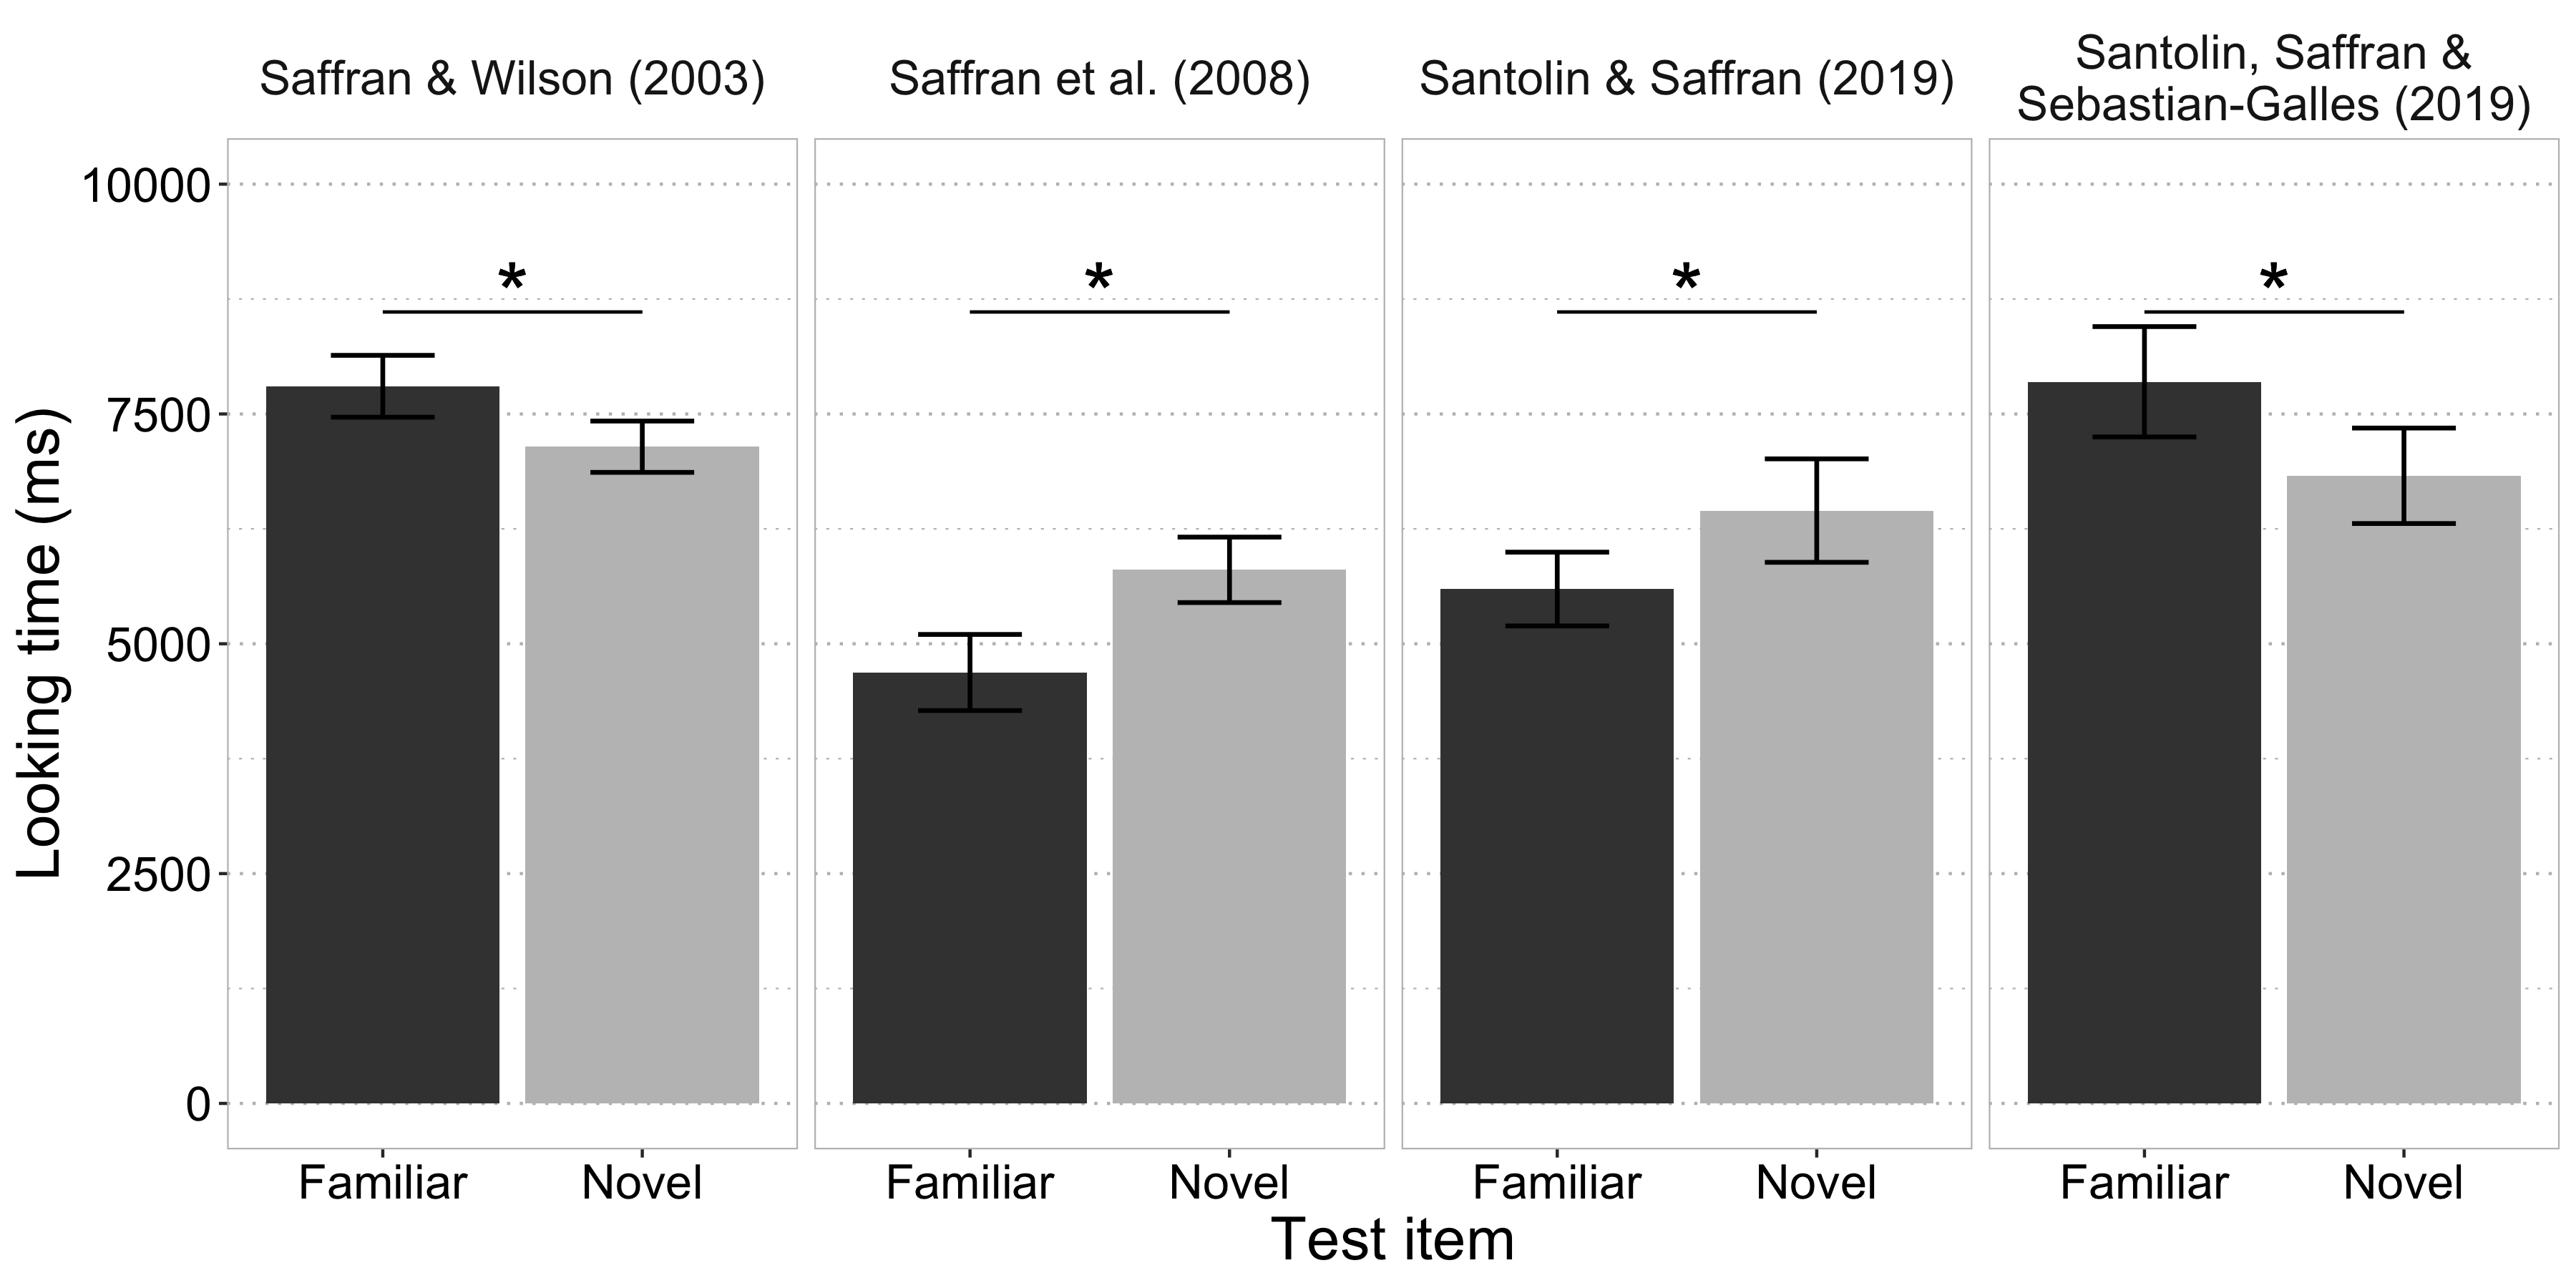
\includegraphics[width=\textwidth]{Figures/01_lookingtimes-study} \caption{Looking time for familiar and novel test stimuli of the original studies. Stimuli vary based on the experiment. Error bars indicate the standard error of the mean.}\label{fig:unnamed-chunk-1}
\end{figure}

\hypertarget{linear-mixed-effect-model}{%
\subsection{Linear mixed-effect model}\label{linear-mixed-effect-model}}

We modeled results of all infants (\emph{N}=102) who participated in the four studies. Number of HPP visits varied from one to six total visits (including the current visit). Since only a small set of infants participated in more than four experiments (\emph{n}=2), we also analyzed the results after reducing our sample to infants who only participated in 1-to-4 experiments, obtaining similar results (see SI, Section 2 for details).

We fit a linear mixed-effect model including \emph{Looking time} as response variable, and \emph{Test item} (familiar vs.~novel), \emph{HPP} (number of experiments conducted with the Head-turn Preference Procedure completed by infants) and their interaction as fixed effects. We also included by-participant and by-study random intercepts (4 levels: Santolin \& Saffran, 2019; its replication; Saffran \& Wilson, 2003; and Saffran et al., 2008). The \emph{HPP} predictor was coded as a continuous variable indicating the overall number of HPP experiments the infants participated in. Familiar test items were coded as baseline. Importantly, the model accounted for cross-participant and cross-study differences in looking time. The rationale behind this choice was that the experiments were similar but not identical, differing in the learning problem and the stimuli used at both familiarization and test. It was therefore reasonable to assume that differences on these dimensions would have affected looking time across studies. Details of the model are provided in SI, Section 3.

We predicted a \emph{Test item} (familiar vs.~novel) by number of HPP interaction, indicating that the duration of infants' looking towards familiar versus novel items would depend on infants' HPP experience. There were at least three possible outcomes: an increase in looking time for novel stimulus, a decrease in looking time for familiar stimulus, or both. We did not have clear expectations on the most plausible scenario.

\hypertarget{results}{%
\section{Results}\label{results}}

We found a statistically significant interaction (\emph{F}(1,100.00) = 11.99, \emph{p} = .001) suggesting that the effect of Test Items on looking time differences was affected by the number of HPP experiments infants had participated in (Table 1, Fig. 2). In line with our predictions, the size of the difference between looking times on familiar and novel test items changed as a function of number of HPP visits. Importantly, results also hold when reducing the data to infants with four or fewer HPP visits (\emph{F}(1,98.00) = 10.43, \emph{p} = .002), indicating that the interaction effect is not driven exclusively by infants with an unusually high number of visits (see SI, Section 4 for details).

We also found a significant main effect of the HPP predictor (\emph{F}(1,133.10\footnote{Degrees of freedom were approximated using the Kenward-Rogers approach, thus sometimes result in non-integers.}) = 4.80, \emph{p} = .030) indicating that the Test Item \(\times\) HPP interaction is mainly driven by a significant decrease in looking time to familiar items as the number of HPP visits increases. There was no evidence that a greater number of HPP visits was accompanied by longer looking to the novel item (\emph{F}(1,133.10) = 0.27, \emph{p} = .606)\footnote{To get this result, the same model was fit coding the novel test item as baseline, as opposed to the familiar item.}.

\begin{longtable}[]{@{}lcccccc@{}}
\caption{\label{tab:unnamed-chunk-2}Summary of the results of the linear mixed-effects model. Degrees of freedom were approximated using the Kenward-Rogers approach, thus sometimes result in non-integers.}\tabularnewline
\toprule
& Coefficient & SEM & 95\%CI & F & Den. df & p\tabularnewline
\midrule
\endfirsthead
\toprule
& Coefficient & SEM & 95\%CI & F & Den. df & p\tabularnewline
\midrule
\endhead
Intercept & 7,679.11 & 673.14 & 6390.13, 9294.12 & 124.69 & 9.06 & \textless{} .001\tabularnewline
Test Item & -1,398.77 & 411.31 & -2204.84, -589.11 & 11.57 & 100.00 & .001\tabularnewline
HPP & -539.70 & 238.69 & -999.88, -74.83 & 4.80 & 133.10 & .030\tabularnewline
Test Item * HPP & 667.11 & 192.64 & 247.23, 1028.51 & 11.99 & 100.00 & .001\tabularnewline
\bottomrule
\end{longtable}

\begin{figure}
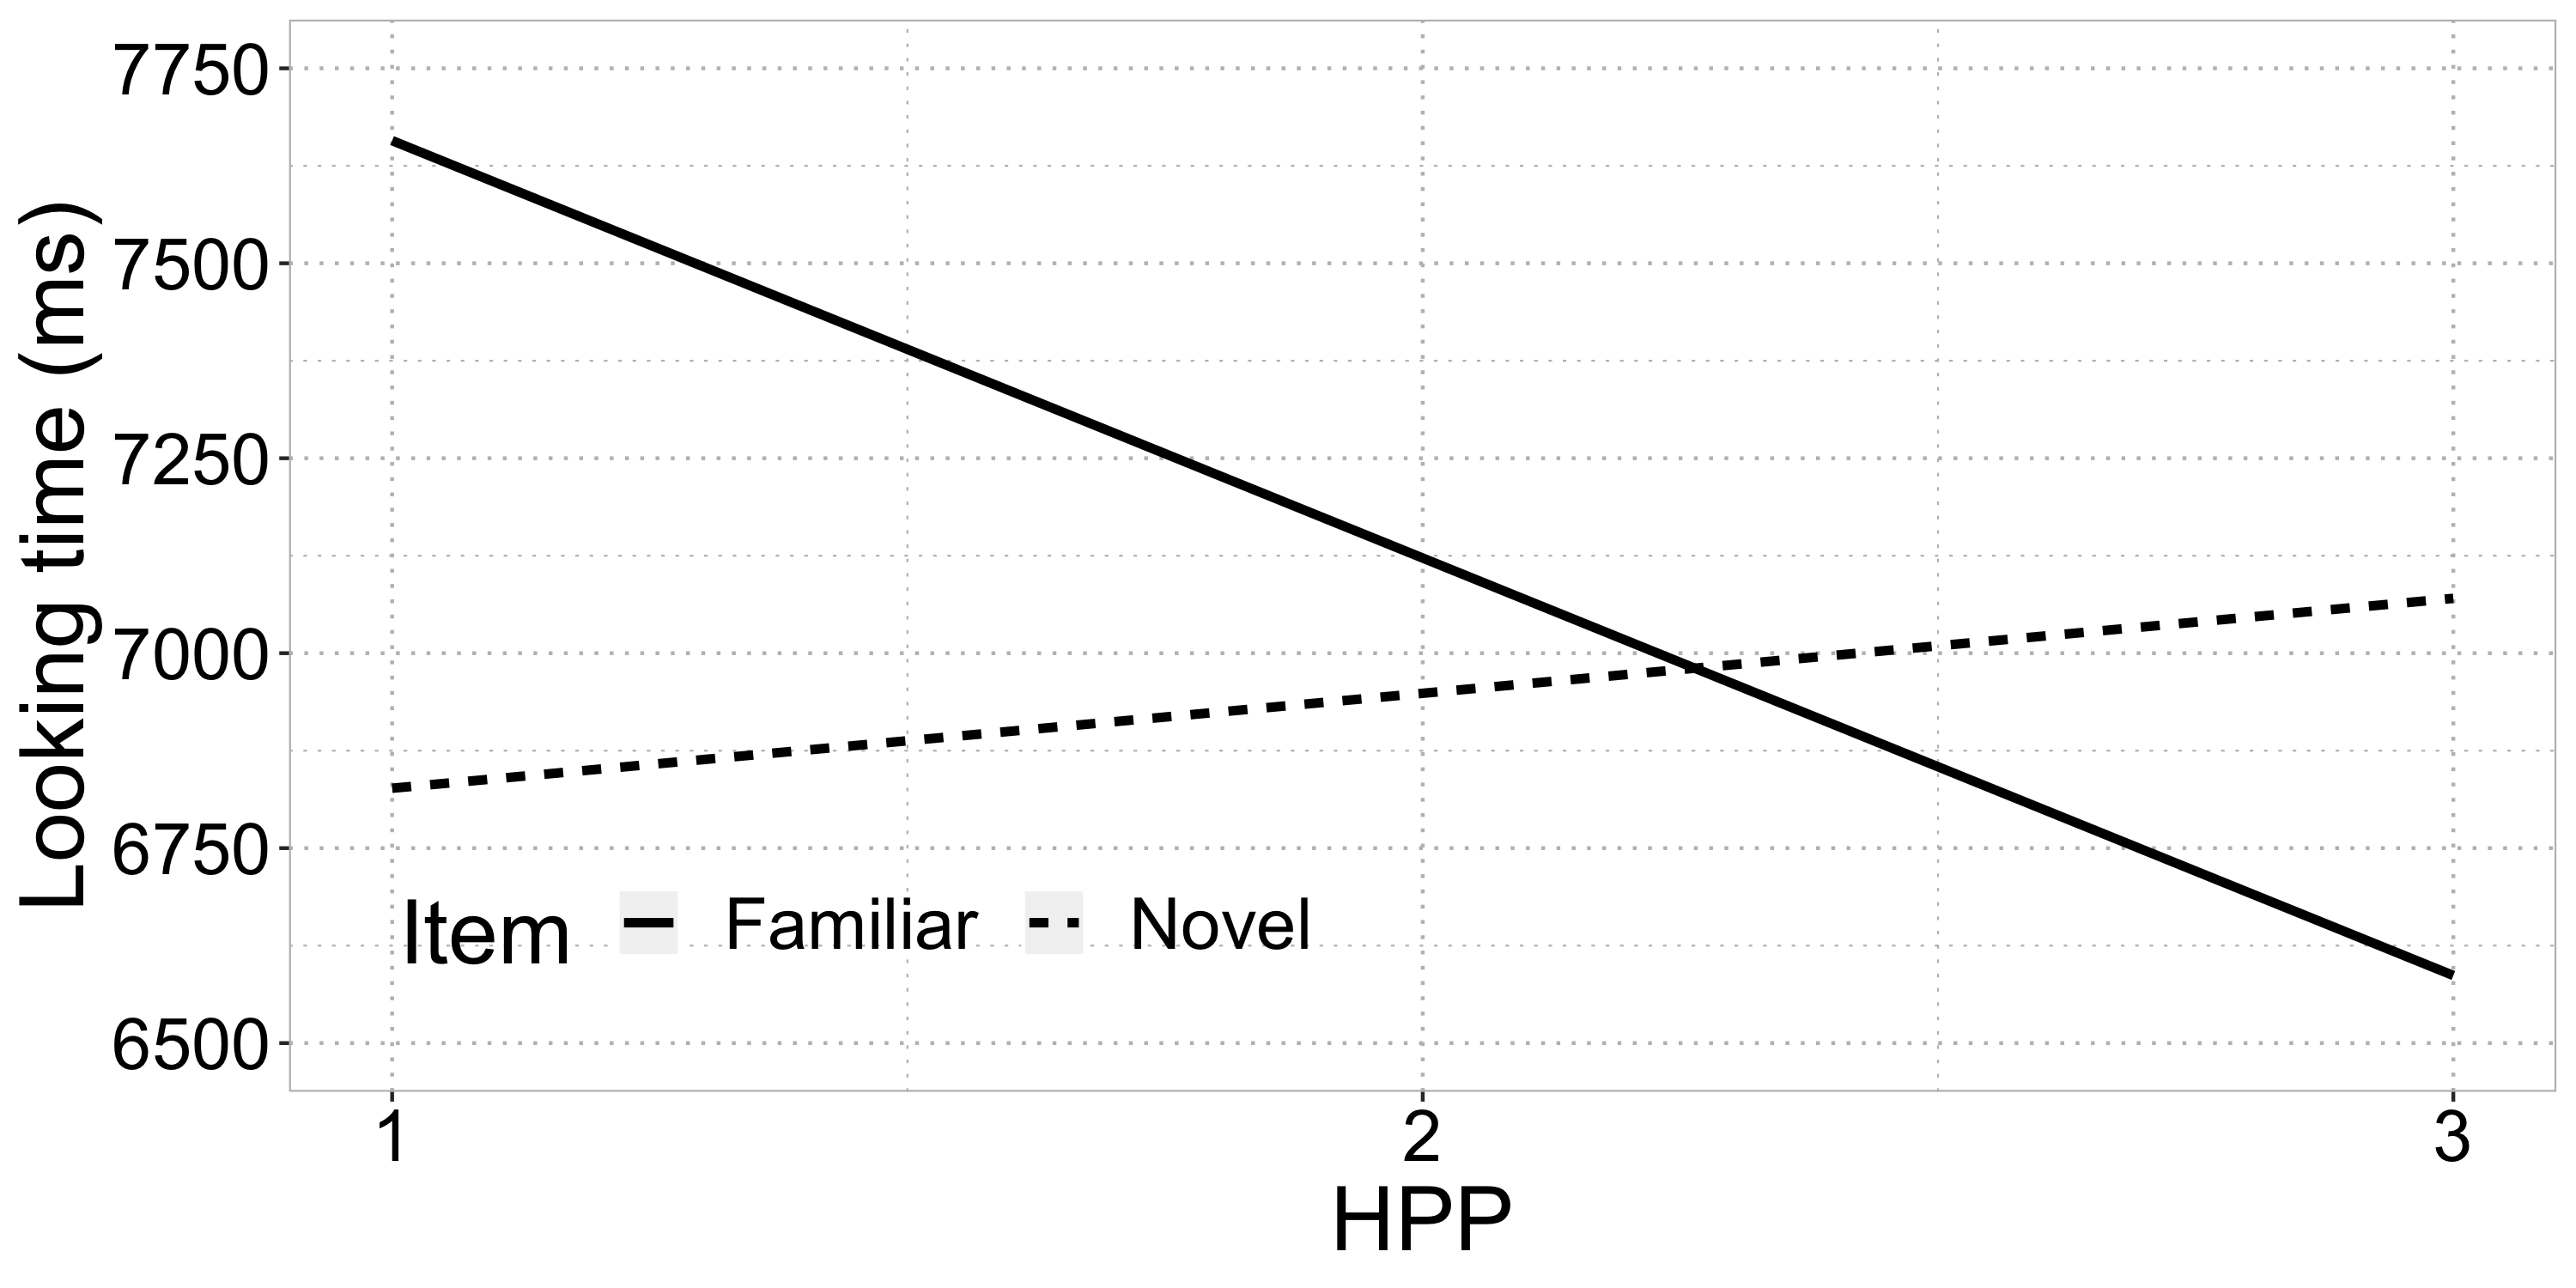
\includegraphics[width=\textwidth]{/Users/GonzaloGGC/projects/Flip/Figures/03_interaction} \caption{Predicted looking time plotted against number of HPP visits. Graph shows an increasing difference of looking time between familiar and novel test items, and a clear drop in looks for the familiar items.}\label{fig:unnamed-chunk-3}
\end{figure}

\hypertarget{discussion}{%
\section{Discussion}\label{discussion}}

Results reported in this article are consistent with our hypothesis that experience with the Head-turn Preference Procedure affects direction of preference. We combined together 4 different experiments with 12-month-old infants performing simple artificial grammar learning tasks, and showed that infants who had not previously experienced the HPP setting were more likely to show familiarity preferences than infants who had prior experience. One possible explanation accounting for such finding relates to the structure of the HPP task. There are at least two types of information that must be simultaneously encoded by the infant at her first HPP experiment: 1) visual-auditory contingency (i.e., sounds appear contingently on the infant looking at the screen), and 2) the experiment stimuli (e.g., word sequences, sound streams). Therefore, infants have to engage in two concurrent learning when experiencing HPP for the first time: learning the structure of the HPP task, and solving the learning problem (e.g., discriminating sound strings following/breaking the grammar patterns). Such double-processing of information likely increases the overall difficulty of the study, biasing results towards familiarity preferences. Infants who return to the lab for subsequent HPP experiments may be more able to focus on the learning problem, resulting in better learning as evidenced in novelty preferences.

It is important to notice that this effect may not just be limited to experiencing the the HPP setting per se, but can be caused by the entire laboratory visit. When infants come to the lab for the very first time, they face a challenging situation: they are moved into a new environment with new people interacting with them, and they enter into testing rooms with a peculiar design (e.g., all-black or all-white walls with big screens) where they are presented with novel sounds and images. This is a great amount of novel information for a young infant to process at once. In contrast, as the infants come back to the lab, location, testing room and research staff may become more familiar, reducing the information load. The present study cannot discern which type of previous experience (HPP setting or lab) is responsible for the observed results.

Our results are consistent with existing theories of cognitive development suggesting that, in spite of their limited capacities, infants 1) constantly gather input from the natural environment, 2) selectively sample the information to learn, and 3) direct their resources to examine the most relevant and informative input (e.g., Bates et al., 1996; Kidd, Piantadosi, \& Aslin, 2014; Saffran \& Kirkham, 2018; Santolin \& Saffran, 2018). Our results suggest that infants actively process information about the lab environment and, consequently, their test performance are affected by how much lab experience they have accumulated. The learning outcome, in fact, seems to be constrained by the amount of novel information infants have to process in parallel when visiting the lab.

Evidence provided in this article has important implications for future interpretation of directions of preference. Infants' prior experience with the lab or a given research paradigm can account for different, and sometimes counterintuitive, patterns of preference. A related hypothesis suggests that less-frequent directions of preference with respect to the pattern of preferences shown in the literature of a given topic (e.g., rule learning) likely represent sign errors as opposed to true infant preferences (Bergmann, Rabagliati, \& Tsuji, 2019; Rabagliati, Ferguson, \& Lew-Williams, 2019). Alternatively, we propose that discrepancies in preferential looking are related to the infants' background of experience with the testing environment (i.e., how familiar is the infant with the lab setting), and, for this reason, such differences seem meaningful and informative about the state of the (infant) learner during a task. However, it is important to notice that our proposed explanation is based on studies measuring discrimination between stimuli as dependent variable rather than direction of preference, as in the above-mentioned papers.

It would be of great interest to investigate the extension of our findings to other preferential paradigms (e.g., infant-controlled preferential looking procedure, visual-world paradigm) as well as other dependent variables. Additional evidence would allow to advance our understanding of how the lab experience modulates infants' performance in a given task, as well as creating an updated model of the factors inducing different patterns of preferences in infant studies.

\newpage

\hypertarget{references}{%
\section{References}\label{references}}

\begin{verbatim}
## Warning in readLines(file): incomplete final line found on 'Flip.bib'
\end{verbatim}

\begingroup
\setlength{\parindent}{-0.5in}
\setlength{\leftskip}{0.5in}

\hypertarget{refs}{}
\leavevmode\hypertarget{ref-aslin2007}{}%
Aslin, R. N. (2007). What's in a look? \emph{Developmental Science}, \emph{10}(1), 48--53. \url{https://doi.org/10.1111/j.1467-7687.2007.00563.x}

\leavevmode\hypertarget{ref-awh2001}{}%
Awh, E., \& Jonides, J. (2001). Overlapping mechanisms of attention and spatial working memory. \emph{Trends in Cognitive Sciences}, \emph{5}(3), 119--126. \url{https://doi.org/10.1016/s1364-6613(00)01593-x}

\leavevmode\hypertarget{ref-bates1996}{}%
Bates, E., Elman, J., Johnson, M. H., Karmiloff-Smith, A., Parisi, D., \& Plunkett, K. (1996). \emph{Rethinking Innateness}. MIT press.

\leavevmode\hypertarget{ref-bergmann2016}{}%
Bergmann, C., \& Cristia, A. (2016). Development of infants' segmentation of words from native speech: A meta-analytic approach. \emph{Developmental Science}, \emph{19}(6), 901--917. \url{https://doi.org/10.1111/desc.12341}

\leavevmode\hypertarget{ref-bergmann_rabagliati_tsuji_2019}{}%
Bergmann, C., Rabagliati, H., \& Tsuji, S. (2019). What's in a looking time preference? \url{https://doi.org/10.31234/osf.io/6u453}

\leavevmode\hypertarget{ref-bosch2001}{}%
Bosch, L., \& Sebastián‐Gallés, N. (2001). Evidence of Early Language Discrimination Abilities in Infants From Bilingual Environments. \emph{Infancy}, \emph{2}(1), 29--49. \url{https://doi.org/10.1207/S15327078IN0201_3}

\leavevmode\hypertarget{ref-colombo1983}{}%
Colombo, J., \& Bundy, R. S. (1983). Infant response to auditory familiarity and novelty. \emph{Infant Behavior \& Development}, \emph{6}(3), 305--311. \url{https://doi.org/10.1016/S0163-6383(83)80039-3}

\leavevmode\hypertarget{ref-dawson2009}{}%
Dawson, C., \& Gerken, L. (2009). From Domain-Generality to Domain-Sensitivity: 4-Month-Olds Learn an Abstract Repetition Rule in Music That 7-Month-Olds Do Not. \emph{Cognition}, \emph{111}(3), 378--382. \url{https://doi.org/10.1016/j.cognition.2009.02.010}

\leavevmode\hypertarget{ref-fantz1964}{}%
Fantz, R. L. (1964). Visual Experience in Infants: Decreased Attention to Familiar Patterns Relative to Novel Ones. \emph{Science}, \emph{146}(3644), 668--670. \url{https://doi.org/10.1126/science.146.3644.668}

\leavevmode\hypertarget{ref-ferguson2018}{}%
Ferguson, B., Franconeri, S. L., \& Waxman, S. R. (2018). Very young infants learn abstract rules in the visual modality. \emph{PloS One}, \emph{13}(1), e0190185. \url{https://doi.org/10.1371/journal.pone.0190185}

\leavevmode\hypertarget{ref-fiser2001}{}%
Fiser, J., \& Aslin, R. N. (2001). Unsupervised statistical learning of higher-order spatial structures from visual scenes. \emph{Psychological Science}, \emph{12}(6), 499--504. \url{https://doi.org/10.1111/1467-9280.00392}

\leavevmode\hypertarget{ref-houston-price2004}{}%
Houston‐Price, C., \& Nakai, S. (2004). Distinguishing novelty and familiarity effects in infant preference procedures. \emph{Infant and Child Development}, \emph{13}(4), 341--348. \url{https://doi.org/10.1002/icd.364}

\leavevmode\hypertarget{ref-hunter1988}{}%
Hunter, M. A., \& Ames, E. W. (1988). A multifactor model of infant preferences for novel and familiar stimuli. In \emph{Advances in infancy research, Vol. 5.} (pp. 69--95). Westport, CT, US: Ablex Publishing.

\leavevmode\hypertarget{ref-johnson2009}{}%
Johnson, S. P., Fernandas, K. J., Frank, M. C., Kirkham, N., Marcus, G., Rabagliati, H., \& Slemmer, J. A. (2009). Abstract Rule Learning for Visual Sequences in 8- and 11-Month-Olds. \emph{Infancy : The Official Journal of the International Society on Infant Studies}, \emph{14}(1), 2--18. \url{https://doi.org/10.1080/15250000802569611}

\leavevmode\hypertarget{ref-jusczyk1995}{}%
Jusczyk, P. W., \& Aslin, R. N. (1995). Infants' detection of the sound patterns of words in fluent speech. \emph{Cognitive Psychology}, \emph{29}(1), 1--23. \url{https://doi.org/10.1006/cogp.1995.1010}

\leavevmode\hypertarget{ref-kidd2014}{}%
Kidd, C., Piantadosi, S. T., \& Aslin, R. N. (2014). The Goldilocks Effect in Infant Auditory Attention. \emph{Child Development}, \emph{85}(5), 1795--1804. \url{https://doi.org/10.1111/cdev.12263}

\leavevmode\hypertarget{ref-rabagliati2019}{}%
Rabagliati, H., Ferguson, B., \& Lew-Williams, C. (2019). The profile of abstract rule learning in infancy: Meta-analytic and experimental evidence. \emph{Developmental Science}, \emph{22}(1), e12704. \url{https://doi.org/10.1111/desc.12704}

\leavevmode\hypertarget{ref-roder2000}{}%
Roder, B. J., Bushneil, E. W., \& Sasseville, A. M. (2000). Infants' Preferences for Familiarity and Novelty During the Course of Visual Processing. \emph{Infancy}, \emph{1}(4), 491--507. \url{https://doi.org/10.1207/S15327078IN0104_9}

\leavevmode\hypertarget{ref-rose2004}{}%
Rose, S. A., Feldman, J. F., \& Jankowski, J. J. (2004). Infant visual recognition memory. \emph{Developmental Review}, \emph{24}(1), 74--100. \url{https://doi.org/10.1016/j.dr.2003.09.004}

\leavevmode\hypertarget{ref-saffran2008}{}%
Saffran, J., Hauser, M., Seibel, R., Kapfhamer, J., Tsao, F., \& Cushman, F. (2008). Grammatical pattern learning by human infants and cotton-top tamarin monkeys. \emph{Cognition}, \emph{107}(2), 479--500. \url{https://doi.org/10.1016/j.cognition.2007.10.010}

\leavevmode\hypertarget{ref-saffran2018}{}%
Saffran, J. R., \& Kirkham, N. Z. (2018). Infant Statistical Learning. \emph{Annual Review of Psychology}, \emph{69}(1), 181--203. \url{https://doi.org/10.1146/annurev-psych-122216-011805}

\leavevmode\hypertarget{ref-saffran2003}{}%
Saffran, J. R., \& Wilson, D. P. (2003). From Syllables to Syntax: Multilevel Statistical Learning by 12-Month-Old Infants. \emph{Infancy}, \emph{4}(2), 273--284. \url{https://doi.org/10.1207/S15327078IN0402_07}

\leavevmode\hypertarget{ref-santolin2018}{}%
Santolin, C., \& Saffran, J. R. (2018). Constraints on Statistical Learning Across Species. \emph{Trends in Cognitive Sciences}, \emph{22}(1), 52--63. \url{https://doi.org/10.1016/j.tics.2017.10.003}

\leavevmode\hypertarget{ref-santolin2019}{}%
Santolin, C., \& Saffran, J. R. (2019). Non-Linguistic Grammar Learning by 12-Month-Old Infants: Evidence for Constraints on Learning. \emph{Journal of Cognition and Development}, \emph{20}(3), 433--441. \url{https://doi.org/10.1080/15248372.2019.1604525}

\leavevmode\hypertarget{ref-santolin2019a}{}%
Santolin, C., Saffran, J. R., \& Sebastian-Galles, N. (2019). Non-linguistic artificial grammar learning in 12-month-old infants: A cross-lab replication study. In. Potsdam, Germany.

\leavevmode\hypertarget{ref-sebastian-galles2009}{}%
Sebastián-Gallés, N., \& Bosch, L. (2009). Developmental shift in the discrimination of vowel contrasts in bilingual infants: Is the distributional account all there is to it? \emph{Developmental Science}, \emph{12}(6), 874--887. \url{https://doi.org/10.1111/j.1467-7687.2009.00829.x}

\leavevmode\hypertarget{ref-thiessen2012}{}%
Thiessen, E. D. (2012). Effects of inter- and intra-modal redundancy on infants' rule learning. \emph{Language Learning and Development}, \emph{8}(3), 197--214. \url{https://doi.org/10.1080/15475441.2011.583610}

\leavevmode\hypertarget{ref-thiessen2005}{}%
Thiessen, E. D., Hill, E. A., \& Saffran, J. R. (2005). Infant-Directed Speech Facilitates Word Segmentation. \emph{Infancy}, \emph{7}(1), 53--71. \url{https://doi.org/10.1207/s15327078in0701_5}

\leavevmode\hypertarget{ref-thiessen2003}{}%
Thiessen, E. D., \& Saffran, J. R. (2003). When cues collide: Use of stress and statistical cues to word boundaries by 7- to 9-month-old infants. \emph{Developmental Psychology}, \emph{39}(4), 706--716. \url{https://doi.org/10.1037/0012-1649.39.4.706}

\endgroup

\end{document}
